\chapter{Entwurf und Implementierung}
\label{cha:implementierung}

\todo{Kapitel-Einleitung}



\section{Modularer Architektur-Vorschlag}

%Komponenten des Brokers.
%
%
%In der CMP: Polling oder Notification?
%
%Was löst eine Aktion aus?
%- Monitoring der Services
%- Änderung der Umgebung
%- User-Aktion
%- Ergebnis einer anderen Policy

\begin{figure}
	\centering	
%	\def\svgwidth{0.95\textwidth}
%	{\tiny
%	\includesvg{images/broker-cycle}}
	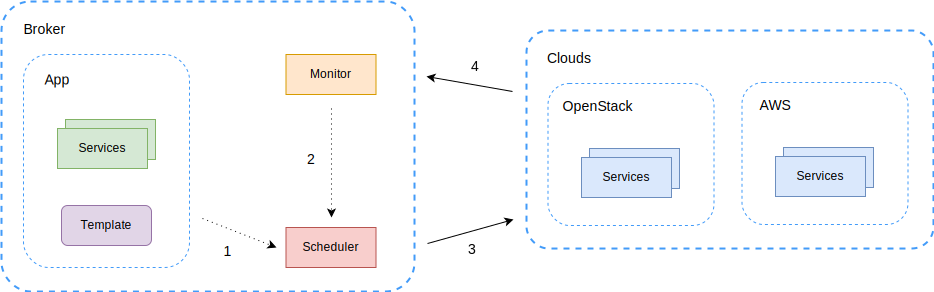
\includegraphics[width=\linewidth]{images/broker-cycle}
	\caption{Arbeitsweise des Multi-Cloud-Brokers als Zyklus: (1) Sammeln der Meta-Informationen alle Cloud-Provider, (2) Sammeln der Laufzeitinformationen der Anwendungen, (3) Sammeln der SLAs, (4) Nutzeränderungen: Neue Anwendungen oder Anpassung von SLAs, (5) Optimierungsplanung, (6) Planausführung auf den Cloud-Infrastrukturen}
	\label{fig:cycle}
\end{figure}

%Zyklus\autoref{fig:cycle}:

%\begin{description}
%	\item[Nummerierte Aufzählung]~\par
\begin{enumerate}
	
	\item Sammeln der Meta-Informationen alle Cloud-Provider
	\begin{enumerate}
		\item Kapazität (CPU, RAM, HDD, Network)
		\item Features (Verschlüsselung, CUDA, …)
		\item Geo-Lokation 
		\item Preis
	\end{enumerate}
	
	\item Sammeln der Laufzeitinformationen der PaaS/Anwendungen
	\begin{enumerate}
		\item Auslastung
		\item Fehler
		\item Ausfälle
	\end{enumerate}
	
	\item Sammeln der SLAs
	\begin{enumerate}
		\item Policy-Definitionen
		\item Policy-Konfiguration
		\item Placement-Algorithmen
	\end{enumerate}
	
	\item Neue Anwendung/Änderung eines SLA
	
	\item Optimierung
	\begin{enumerate}
		\item Feste Vorgaben (Geo, Backup)
		\item Weiche (Preis, Latenz, Verfügbarkeit)
	\end{enumerate}
	
	
	\item Ausführung
	\begin{enumerate}
		\item Netzwerkkonfiguration
		\item Allokation/De-Allokation von Ressourcen
		\item Deployment
		\item Migration
		\item Logging/Benachrichtigung
		\item Backup
	\end{enumerate}
	
\end{enumerate}

\section{Brokering}


%https://de.wikipedia.org/wiki/Constraintprogrammierung
%https://de.wikipedia.org/wiki/Scheduling

%entailing multiple constraint satisfaction (MCS)
%
%\todo{Schaubild, was wird wann gematcht}
%% Pseudocode des Algorithmus, wie in Meryn
%
%Kostenoptimierung
%
%Preisentwicklung? 
%
%Migration je nach Tageszeit? 
%
%Kosten der Datentransfers 
%
%Subscription On-Demand/Monthly/Yearly 
%
%Kompliziert durch undurchsichtige Staffelpreise
% https://www.rightscale.com/blog/cloud-cost-analysis/aws-vs-azure-vs-google-cloud-pricing-compute-instances

%https://www.rightscale.com/blog/cloud-cost-analysis/comparing-cloud-instance-pricing-aws-vs-azure-vs-google-vs-ibm

%
%Cost Calculators 
%
%http://go.appscale.com/cloud-cost-calculator-help 
%
%https://github.com/ifosch/accloudtant 
%
%https://awstcocalculator.com/# 
%

\section{Testumgebung: OpenStack \& Hyrise-R}

Hyrise\footnote{\url{https://hpi.de/plattner/projects/hyrise.html}} ist eine In-Memory-Forschungsdatenbank der Fachgruppe \emph{Enterprise Platform and Integration Concepts (EPIC)} am Hasso-Plattner-Institut \cite{grund:2010:hyrise}. Die Datenbank teilt sich einige Eigenschaften mit \emph{SAP HANA}\footnote{\url{https://www.sap.com/products/hana.html}}: Ein \emph{Delta Store}, spaltenorientierte Speicherung, Wörterbuchkodierung und weitere Komprimierungstechniken sowie den \emph{Insert-Only}-Ansatz und Partitionierung. Herausragend ist die OLAP-Performance, enthalten sind aber auch Optimierungen für OLTP-Aufgaben.

Hyrise-R ist eine Erweiterung des Basisprojektes um Replikation \cite{schwalb:2015:hyrise-r}. Es folgt dabei dem \emph{Scale-Out}-Ansatz: Alle schreibenden Operationen werden auf einem einzigen \emph{Master-Node} durchgeführt. Dessen Datensatz wird in weniger als einer Sekunde (\emph{lazy}) mit beliebig vielen \emph{Replica-Nodes} abgeglichen. Diese Spiegelungen bearbeiten alle reinen Leseanfragen und machen den Verbund so skalierbar, siehe \autoref{fig:hyrise-r}. Nach dem \emph{CAP-Theorem} sind Verfügbarkeit und Partitionstoleranz hier also wichtiger als Konsistenz. 

	\begin{figure}[ht]
	\centering
	\def\svgwidth{0.95\textwidth}
	\includesvg{images/hyrise-r}
	\caption{Verteilte \emph{Hyrise-R}-Architektur mit getrennter Verarbeitung von Lese- und Schreibanfragen. Der Master-Knoten dient als \emph{Single Source of Truth}. Zur Leistungssteigerung übernehmen Spiegelserver die Beantwortung der meisten Leseanfragen. Kleinere Inkonsistenzen werden dabei in Kauf genommen. Aus \cite{ssiclops:d42:experiments-measurements}.}	
	\label{fig:hyrise-r}
\end{figure}

Durch die verteilte Architektur ist Hyrise-R ein potenzieller Kandidat als Testanwendung innerhalb der Multi-Cloud-Umgebung. Einige \emph{SSICLOPS}-Teilprojekte untersuchten bereits Zuverlässigkeit, Performance, Datensicherheit und Vertraulichkeit in einer privaten OpenStack-Föderation \cite{ssiclops:d23:security-extensions, ssiclops:d42:experiments-measurements, bastian:2017:openstack-policies}. \todo{Diagramm:Hyrise-R on SSICLOPS}

Im Rahmen dieser Arbeiten sind einige Infrastrukturteile als Code veröffentlicht: So existiert zum Beispiel eine Docker-Teststellung mit grafischem Cluster-Manager, um die Performance bei verschiedenen Replikationsstufen zu prüfen. Diese Infrastruktur wurde in mehreren Studienarbeiten weiter angepasst, um Hyrise-R-KVM-Images in OpenStack bereitzustellen \cite{eschrig:2016:ssiclops-masterproject, maschler:2017:ssiclops-masterproject}. Möglicherweise können Teile dieser Arbeiten weiterentwickelt werden.


\input{content/4-4_openstack-testbed.tex}

\input{content/4-5_devstack-docker.tex}

\input{content/4-6_multi-cloud-bibliotheken.tex}


\section{Entwicklungsumgebung}

% Hyrise-R-OpenStack- und Docker-Images, wie ersxtellt?

%Bestehende verteilte Anwendungen für den EInsatz in der CLoud vorbereiten, STichwort CLoud Native.
%Ausgangslage? Git-Repository mit teilautmatisierten Shell-Skripten und Makefiles. Automatisierung der Build, Test und Produktions-Infrastruktur, Ubuntu 16.04 auf Bare-Metal, VM und (Docker)Container.
%Integrieren der bestehenden Tests in diese Umgebungen.
%Packen des Geamtpakets aus Ausführungsumgebung, Programm und (Test-)Daten. auch automatisiert. Die Konfiguration ist variabel. SIe wird schematisch in der App-Konfiguration vorgegeben und dann von der CMP während der initialen Bereitstellung oder späteren Re-Deployments angepasst und ausgeführt.

% Tatsächliche Broker Architektur
% Code-Eigenheiten
% Tests/KPIs/Validierung der Hypothese

\section{Softwarearchitektur}

%as in Grozev 42: Federated CLoud Management: There is a central repository of images. this is replicated to the specific iaas/caas providers on demand.
%
%Alle weiteren Managementprozesse sind für Clients transparent.


\section{Multi-Provider-Service-Schema}

% D2.1: Übersicht Policy-Sprachen: Performance und Speichergröße. Entgegengesetzte Interessen. Lesbarkeit über zweiteiliung: Einmal für Menschen, einmal auf Bit-ebene für Maschinen. SLA über Proxy

%D2.2: Policys auf allen Schichten

%Matthias Bastian: Policy in OpenStack.

...und SLAs.

Ziel: Portabilität.

Mensch-und maschinenlesbar

YAML als aktuellen Standard

%TOSCA komplex, aber vielversprechend. Hierauf aufbauen (eigenen YAML-Entwurf erwähnen) und Brokering hinzufügen. Hier muss festgelegt erden, welcher Service-Teil auf welchem Provider mit welchem Instanz-Typen bereitgestellt werden soll. Dies soll automatisiert anhand von SLA/Policy und Preis entschieden werden. Unterstützt TOSCA deklarative Service-Definitionen?
%
%
%TOSCA hat folgendes nur optional
%- YAML (als SimpleVersion)
%- Multi-Provider als Plugin (nicht gewartet)
%- 
\begin{listing}[ht]	
	\inputminted[]{yaml}{./src/provider.sample.yaml}
	\caption{Provider-Definition und Zugangsdaten. Der Broker liest alle eingetragenen Accounts automatisch ein und berücksichtigt sie bei der initialen Service-Bereitstellung sowie in Optimierungsläufen. Public-Clouds benötigen nur Zugangsdaten wie Benutzername und Passwort -- alle weiteren Informationen erfragt der Broker dynamisch zur Laufzeit vom Provider. In Private-Cloud-Umgebungen ist dies nicht immer möglich: Details zur Verfügbarkeit, geografische Lage und Kosten müssen manuell eingepflegt oder vom Monitoring festgestellt werden.}
	\label{listing:provider}
\end{listing}



Platzhalter werden mit Jinja während des Deployments gefüllt.

Ablage der Pläne als Dokumentation.

Broker durch Metainformationen (und Labels) der Instanzen theoretisch zustandslos -> Broker selbst ist nicht ausfallgefährdet.

Erklärung der Metainformationen (versionierbar), verschiedenen Parameter und Rollenbeschreibung.

Je Provider Angaben zu Image und Startkommando. Dies wird hier eingetragen, um vom Broker dynamisch mit aktuellen Variablen angepasst zu werden: IP, Port...

Abhängig vom Service Level: IaaS/CaaS. Auch PaaS ist so denkbar. (Angabe als Image, Interpretation durch den Broker)

Beispiel verlinken.
Kapitel: Legacy Services Hyrise

Image-Erstellung und Repository.

Eigene Befehle
- Cloud-Init (Standard)
- shell/bash (Docker)

Vordefinierte Policys z.B. zum Verhalten im Fehlerfall. Aber auch Zusatzinformationen: Wie ist die Zustandsprüfung auf Service-Ebene auszuführen. Wichtig für Monitoring der Verfügbarkeit (SLA).

Abhängigkeiten von Services und wie oft global vorhanden? Hier: global ein master, abhängig vom Dispatcher.

\begin{listing}[ht]	
	\inputminted[firstline=15]{yaml}{./src/hyrise-r.sample.yaml}
	\caption{Providerübergreifende Servicevorlage. Der Ausschnitt zeigt die Definition des zentralen \emph{Hyrise-R-Dispatcher}-Dienstes. Nicht zu sehen sind Metadaten und die übrigen Anwendungsbestandteile. Parameter werden zur Laufzeit vom Broker eingesetzt.}
	\label{listing:hyrise-r}
\end{listing}

Könnte auch zu einem konkreten CAMP-Plan umgewandelt werden. So wie TOSCAMP. Stattdessen nur ein Template Schema und Graph zur Laufzeit.
%https://brooklyn.apache.org/v/latest/blueprints/setting-locations.html


\section{Tests und Diskussion}

%Kosten: Rechenzeit und Bandbreite (außerhalb einer Cloud) also gegenläufiges Ziel zu Portabilität und Ausfallsicherheit, denn die geringsten Kosten fallen bei dem Betrieb in einer einzelnen Cloud eines Providers an.
%i) providers’ pricing models, (ii) application’s communication patterns and (iii) distribution of nodes over providers.
%https://www.google.de/url?sa=t&rct=j&q=&esrc=s&source=web&cd=1&ved=0ahUKEwju27vHs6DZAhUCWRQKHRv7BEcQFggrMAA&url=http%3A%2F%2Fwww.mikesmit.com%2Fwp-content%2Fpapercite-data%2Fpdf%2Fcloud2012.pdf&usg=AOvVaw3e6yhHYmhWBbIxtr7MqkuX

%verschiedene OpenStack-Versionen haben unterschiedliche Schnittstellen. Auch dies kann über die Middleware abgefangen werden. RefStack testet API, Rally testet performance und führt tempest-Tests aus.


Aufwand einer Multi-Cloud-Strategie

Umsetzung der Policys

Potential

Vorteile durch Multi-Cloud-Bibliotheken

Aufwand für ein Multi-Cloud-Testbed